
This section will attempt to introduce some broad and fundamental ideas, ultimately rediscovering some key aspects of what is known as \say{process philosophy}.

To begin, we will develop the problem's context, drawing on work from a variety of fields, including cognitive science, computer science, mathematics, philosophy, and political economy.
In addition, we will look at past and current events to attempt to bring the current historical moment into focus.

\bigskip

Our argument will proceed as follows.
First, we will attempt to view the problem of human social organization through the lens of resources and communication.
Then, we will describe a fundamental link between representation and computability.
We will then turn to the role of analysis in society, and discuss ways in which analysis can fail.
Next, we will connect ideas from philosophy and cognitive science, casting light on an important property of subjective mental concepts.
Finally, we will argue that pairwise preferences are well-suited to the task of representing subjective preference, supporting this argument with the analysis of a number of applications.

\subsection{A Schematic View}

\begin{center}
\begin{quotation}
\textit{Man is not an ant, conveniently equipped with an inborn pattern of social instincts.
	On the contrary, he seems to be strongly endowed with a self-centered nature.
	If his relatively weak physique forces him to seek cooperation, his inner drives constantly threaten to disrupt his social working partnerships.}
\end{quotation}
	- Robert Heilbroner, \textit{The Worldly Philosophers}, p18
\end{center}

Let us consider the problem of nonviolent coordination at scale.
Specifically, let us view this is a problem of preference resolution.
Let us view preference resolution as a problem of information flow.

Small communities, such as groups of friends, information flows easily across the human medium of language, and these communities are generally seen as capable of peaceful, mutually-beneficial coordination.
They resolve preferences easily, with few resources, and the results are generally satisfactory \cite{deacon}.

As communities grow larger, the amount of total information increases and preferences become more complex and difficult to resolve.
Further, language loses efficiency as meaning fluctuates across the group.
This increase in problem scale and decrease in language efficiency lead to a need for some form of new structure to manage this process and coordinate the members \cite{hobbes}.
Structures require additional resources, or a more efficient utilization of existing resources.
If the community cannot acquire new resources or technology, we can expect the nature of coordination to become more oppressive, at least for some members of the community \cite{eisenberg}.

The use of the term \say{non-violent} might (reasonably) seem to suggest that its absence implies violence; we choose to interpret it less dramatically as a loss of personal freedom.
Consider a bleak workplace, in which workers have relatively little control over their work \cite{lin}.
Consider a bronze-age empire, in which large public works projects were built by coercing large segments of the population into service \cite{heilbroner}.

This is the schematic relationship: scale and nonviolence are opposed, given a fixed level of resources and technology.
Additional resources or more efficient structure can allow nonviolent coordination at a larger scale.
\say{Structure} can refer to both objective social forms (such as democratic institutions), as well as the organization of mental concepts (such as the notion of \say{democracy}).

This last century has seen great advances both in terms of resources and technology.
The majority of our existing preference-resolution structures predate these developments.
In light of this, it would seem reasonable that there exist some number of viable preference-resolution frameworks waiting to be developed.
Experiments in developing these frameworks, falling under the banner of \say{liquid democracy}, are ongoing.
Recent success includes the use of pol.is in Taiwan \cite{barry}.
In this example, pol.is was used as part of the \say{vTaiwan} initiative to gather fine-grained public opinion to inform the legislative process.

It is just such a framework that we will attempt to develop.
We will study it using standard tools and evaluate its merits objectively.


\subsection{Representation}

Our modern base-10 numbering system, commonly known as the \say{Arabic} numbering system, has roots in in both the Middle East and India.
Originally developed in India, this numbering system was brought to the Middle East by (among others) the 9th-century Persian mathematician Al-Khwarizmi, via his \textit{On the Calculation with Hindu Numerals}.
Fibonacci, a 13th-century Italian mathematician, became aware of this text and became an advocate for this numbering system, arguing for its adoption in place of Roman numerals in his \textit{Liber Abaci} \cite{ore} \cite{ferguson}.

Prior to the adoption of Arabic numerals, mathematics was done using Roman numerals \cite{heilbroner} \cite{gowers}.
Roman numerals, while adequate for counting and basic addition and subtraction, were unwieldy for more complex operations like multiplication and division; hence the widespread use of the abacus as a computational tool.
To practitioners of this era, such operations would likely have been seen as \say{advanced}; problems involving these operations would have been \say{difficult}.
The adoption of the Arabic system allowed for previously challenging analysis to be performed quickly, easily, and accurately; leading to an overall acceleration in the pace of mathematical development.
In the parlance of machine learning, we could argue that the abacus represents an optimization within a local optimum; the adoption of the new numbering system represents an escape from that optimum.
In this historical anecdote, we see a demonstration of a fundamental relationship: that between \textbf{representation} and \textbf{analysis}.
Analytical methods are defined in relation to one or another representation; changes in representation imply a change in the set of available analytic operations.
In addition, observe that changes in representation have no impact on the underlying world; nothing about the world changed to make multiplication easier.
Change occurred only in the mind.

The study of this type of history of thought came into popularity during the 20th century, best exemplified by the work of the post-modern philosophers.
Michel Foucault was the first to attempt an \say{excavation} of our culture, an effort to detect the hidden history of our understanding \cite{foucault}.
Thomas Kuhn achieved a parallel, if not more impressive, excavation of science, showing how the idealized perfection of the objective scientific method fails when implemented by human beings \cite{kuhn}.

\bigskip

The notion of transforming from one representation to another appears often in the computer science and industrial engineering literature; in the former, pertaining to problems and the algorithms which solve them, and in the latter, to optimization.
Often, abstract notions of representation have concrete implications in terms of computability; this will become a key theme moving forward.
In computer science, a problem is said to \textit{reduce} to another if it can be shown that an instance of the first can be transformed into an instance of the second, while preserving truth conditions.
An problem that may be difficult to analyze in one form may become easy to analyze if converted into a different, but provably equivalent, form.
In optimization, there exists tremendous knowledge on how to solve certain kinds of optimization problems, if represented in specific constrained (convex) forms.
Problems defined as optimizations of convex objective functions over convex sets can be solved by computer relatively quickly and precisely.
Much of the skill in this field is being able to identify how a problem represented in some (arbitrary) form can be transformed into an equivalent convex optimization problem (such as a linear, quadratic, or semidefinite program).
The ability to discern these relationships among problems is a fundamental skill for researchers in these fields.

\bigskip

As observed by British computer scientist Philip Wadler \cite{wadler}: 

\begin{quotation}
\textit{
	Powerful insights arise from linking two fields of study previously thought separate.
	Examples include Descartes's coordinates, which links geometry to algebra, Planck's Quantum Theory, which links particles to waves, and Shannon's Information Theory, which links thermodynamics to communication.
	}
\end{quotation}

For a more current example, we can look at recent development in machine learning.
Graphical models, a formalism for representing and analyzing complex joint probability distributions as graphs, allowed for the mixing of analytic techniques from both statistics and computer science.
Problems that are difficult to solve for a probability distributions are may be easy to solve for an equivalent graph, and vice versa \cite{wainwright}.

An important clarification is that for problems which can \textit{in principle} be solved in several representations, one representation may allow for \textit{faster} solutions.
This is important because problems requiring hours or months of computation to solve are essentially unsolvable for applications needing results in minutes or days.

An interesting (but speculative) example comes to us via studies of the Wason selection task.
In this task, participants are asked to solve logical reasoning problems by flipping cards.
Experiments have shown that such problems are difficult when presented abstractly, but become significantly easier when presented in terms of common social reasoning tasks \cite{cosmides}.

\bigskip

We can extend this notion of representation and analysis to more general domains.
Natural language is a representation; the written word can be read, but not analyzed with the precision of mathematics.
Images, music, and so on are also representations; each representation permits some modes of analysis and eliminates others.

In machine learning and optimization, it is very common to represent data as points in high-dimensional space.
A car, possessing \textit{weight, acceleration, horsepower, mpg}, and \textit{year}, can be thought of as a point in five-dimensional space, denoted $\mathbb{R}^5$ (more specifically, in the positive orthant of this space, $\mathbb{R}^5_+$).
Such representations allow for analysis using all of the tools of geometry and linear algebra.
These tools are powerful; much research has been conducted on methods for \textit{embedding} non-numeric data types into these types of space.
Examples of such techniques include collaborative filters and word vectors \cite{mikolov} \cite{koren}.

The above discussion has been qualitative; let's place the concepts of representation and analysis on more rigorous footing.


\subsection{The Data Processing Inequality}

One of the first results in the field of Information Theory goes as follows:

If you have three variables, $\{X, Y, Z\}$, existing in a Markov relationship such that $X$ affects $Y$, and $Y$ affects $Z$:

\[
X \rightarrow Y \rightarrow Z
\]

Then the \textit{mutual information} (intuitively, the amount one variable tells you about another) between $Z$ and $X$ can never be more than the mutual information between $Y$ and $X$.
This is known as the \textit{data processing inequality}\cite{cover}, because we can think of $X$ as some sort of \say{true} world, $Y$ as some data (measurements) taken of the world, and $Z = f(X)$ is the result of some analysis process $f$ we perform on those measurements.
The data processing inequality states that no amount of analysis can produce information about the world not already present in the data itself. This can be stated formally as:

\[
I(X; Y) \geq I(X; Z)
\]

At first glance, this may seem incorrect.
After all, what is the point of data analysis if we can't learn anything new?
To understand why this makes sense, we need to think of an analysis $f$ not as providing new \textit{information}, but rather as taking existing information and \textit{converting} it into a more applicable form.
Consider an average over $n$ measurements:

\[
f(X) = \frac{1}{n} \sum_{i=1}^n X_i
\]

The average contains less \textit{information} than the original data (for example, by discarding all information concerning variance), but is nonetheless a concise and useful summary of an important aspect of the data.

\bigskip

This result has several implications.
First, it allows us to frame the general problem of optimization and machine learning as the exploration of the space of possible data analyses.
To illustrate this, let us present the data processing inequality in the language of machine learning:

\[
Y \rightarrow X \rightarrow \hat{Y} \Rightarrow I(X; Y) \geq I(\hat{Y}; Y)
\]

Here, we have the standard notation of $Y$ representing the true, unobservable world; $X$ represents some data set of measurements taken from that world, and $\hat{Y} = f(X)$ representing the result of some analysis $f$, which may be, among other things, prediction, classification, or structural description of the data $X$.

Problems in optimization and machine learning are generally represented in a common form: we have some goal, represented via a real-valued \textit{objective function}.
This objective function (also known as as \textit{loss function}) calculates some key metric, like the likelihood of a prediction or the magnitude of an error.
With this function, we can then test various candidate data analyses and see how they perform with regard to this metric.
The analysis which does the best (by minimizing or maximizing the metric) is our answer.
Formally, if we think of $L$ as our objective function, and $f$ being the analysis, then we are looking for an optimal analysis $f^*$ such that:

\[
L(f^*(X)) \geq L(f(X))
\]

$\forall f \in \mathcal{F}$, with $\mathcal{F}$ representing the set of all possible analyses.
When $L$ is some type of error metric, we are likely optimizing some (potentially convex) function.
When $L$ is a type of likelihood, we are likely performing some form of statistical parameter estimation.
The role of $L$ is important, in that it is often the derivatives of $L$ that allows us to explore $\mathcal{F}$.
Much research in these fields can be seen as concerning itself with 1) developing new methods for exploring $\mathcal{F}$, and 2) developing new functions $L$ to facilitate progress with (1).

\subsection{Measurement}

Ultimately, our goal is knowledge: information about the world.
When speaking of measurement, we treat the term very generally. Taking the temperature with a thermometer, tagging animals in wildlife preserves, and writing essays can all be seen as efforts to represent symbolically some aspect of the world.
A first key idea is that measurement and representation are fundamentally linked; a measurement is only interpretable as a form of symbolic representation.
A second key idea is that advances in measurement fundamentally expands the space of possible analyses; conversely, the power of analyses is upper-bounded by the power of measurement.

For an historical example, consider the history of oncology.
In attempting to study cancer, progress was made most rapidly for Leukemia, largely due to the ease with which cancer could be measured in the blood \cite{mukherjee}.

For a timely real-world example, consider the ubiquity of mobile phone cameras and the influence such cameras have had on police accountability.
Ostensibly, police have been abusing minority populations for decades, if not for centuries or even millennia.
Progress on this issue was slow, in large part due to difficulty in measuring the problem.
Soon after mobile phone cameras became commonplace, reporting (measurement) of police violence increased dramatically, giving rise to national protest and the well-organized and influential Black Lives Matter movement.
In this example, it is easy to see how the critical factor was change in the underlying world, nor exclusively the development of better organizing techniques, but rather innovations in methods of measurement.

\bigskip

Formally, let us think of a representation $r \in \mathcal{R}$ as a process applied to the world $Y$, resulting in some objective measurement (data) $X \triangleq r(Y)$.
The world is always at least as complex as the measurement (consider the example of a map vs a territory: a perfect map would necessarily be the size of the entire territory).
This means than all measurements are information-discarding.
This means that we can compare two measurements $r^*, r \in \mathcal{R}$ by comparing their mutual information.
If $r^*$ captures more information, then:

\[
I(Y; r^*(Y)) > I(Y; r(Y)).
\]

If would prefer to think of $r$ as a random function (to incorporate the notion of measurement error), then the relation becomes:

\[
I(Y; \mathbb{E}[r^*(Y)]) > I(Y; \mathbb{E}[r(Y)]).
\]

We cannot actually evaluate $I(Y; r(Y))$, as $Y$ is not available for analysis except through $r(Y)$; it is necessarily a unknowable object.
This does not, however, mean that $r$ is beyond study.
Rather, we will evaluate $r$ indirectly, by seeing how it impacts downstream analysis.
The key point is that it may always be possible to find a better $r^*$; \textit{the existence of such an $r^*$ cannot be disproven.}

\bigskip

Recalling the data processing inequality and our historical examples, we see how transforming between representations does not increase information; rather, it allows for new kinds of analysis of existing information.
We can think of the process of transformation as applying a function

\[
g: X \rightarrow X^\prime
\]

$g \in \mathcal{G}$, which maps representation $X$ to $X^\prime$.
If this function is \textit{injective} (or \say{one-to-one}), then both representations contain the same amount of information.
The conversion between graphs and matrices is an example of this type of transformation.
If the function is not injective, then information will be lost during the transformation.
This transformation may still be desirable (and often is) if the target representation allows for more valuable task-specific analysis.
The conversion of natural language into a bag of words is an example of this type of transformation.

Formally, we can say that

\[
I(Y; X) \geq I(Y; g(X))
\]

$\forall g \in \mathcal{G}$. With this result in hand, it may seems like transforming between symbolic representations is pointless.
However, it may be the case that a transformed representation permits analysis in away the original does not.
Analysis of text often falls in this category.
Many techniques for textual analysis rely on conversions of large blocks of text into many small entities: either single words (bags of words) or local word groups (n-grams).
These entities are then counted, and the statistical properties of these counts are analyzed.
These types of analyses have yielded valuable results: Markov models of language and topic models are just two examples \cite{blei}.
We can also think about recommendation systems, in which individuals and items are typically embedded into high-dimensional Cartesian space, as a type of representation transformation \cite{koren}.

The utility of these models is hard to capture in the language of mutual information, as it is always true that:

\[
I(Y; r(Y)) \geq I(Y; g(r(Y))) \geq I(Y; f(g(r(Y))))
\]

To represent the utility of task-specific analysis, we will posit a task-specific \textit{utility function} $U_t$, whose domain is any arbitrary analysis, and range is $\mathbb{R}$.
This utility function is left intentionally general and can incorporate many factors, such as computability.
The subscript $t$ reflects the notion that utility is interpreted as a function of time (or more concretely, computer instructions).

For a concrete example, let us consider the classic problem of sorting.
Consider an unsorted array $X$ of $n$ integers, which we would like to sort.
We will compare two algorithms: insertion sort, denoted $f_i$, and quicksort, denoted $f_q$.
As insertion sort runs in time $O(n^2)$ and quicksort runs in time $O(nlogn)$, we can say that:

\[
U_{O(nlogn)}(f_q(X)) = U_{O(n^2)}(f_i(X))
\]

Further, we can say that:

\[
U_{O(nlogn)}(f_q(X)) \geq U_{O(nlogn)}(f_i(X))
\]

This example illustrates another important point: although we introduce $f$ as a very general function, utility is evaluated only on concrete implementations.
Observe that an analysis $f \in \mathcal{F}$ assumes a particular representation as input; we make our notation more precise by subscripting: $f_g \in \mathcal{F}_g$.

For a second concrete example, let us consider the basic problem of indexing.
We have a linked list $X$ of $n$ elements, and will need to repeatedly access arbitrary elements by position.
We have three functions: $g_{la}$, which converts a linked list to a contiguous array, $f_l$, which indexes over a linked list, and $f_a$, which indexes over an array. $g_{la}$ has complexity $O(n)$, $f_l$ has complexity $O(n)$, and $f_a$ has complexity $O(1)$.
We can see that, for a single access:

\[
U_{O(n+1)}(f_a(g_{la}(X))) = U_{O(n+1)}(f_l(X))
\]

If we need to access elements $k$ times, however, we will find that (assuming that $g_{la}(X)$ is evaluated only once):

\[
U_{O(n+k)}(f_a(g_{la}(X))) = U_{O(nk)}(f_l(X))
\]

We see how the transformation of representation can yield benefits in terms of utility over time.
Complexity analysis is nothing new; the value of this notation is the easy extension to approximate algorithms, which converge arbitrarily close to the \say{true} answer over time.
This notation also allows us to compare different classes of algorithms.
In image recognition, for example, deep neural networks have been shown to outperform most other algorithms, in terms of classification accuracy
These algorithms, however, are relatively slow to train.
$U_t$ allows us to compare these algorithms in a new way: a neural network might have more utility over a long time horizon, but a simpler algorithm could have higher utility if time were limited.

The problem is therefore one of finding a transformation and analysis \textit{pipeline} $f_g^*$ such that:

\[
U_t(f_g^*(X)) \geq U_t(f_g(X))
\]

$\forall f_g \in \mathcal{F}_g$.

In optimization, for example, problem constraints are often \say{relaxed} to allow for fast solutions which assume convexity.
We can think of these relaxations as information-discarding transformations which increase \textit{overall} utility by allowing for fast analysis.
Incorporating notation from earlier, we are ultimately interested in functions $r^*$ and $f_g^*$ such that:

\[
U(f_g^*(r^*(Y))) \geq U(f_g(r(Y)))
\]

$\forall r \in \mathcal{R}$,  $\forall f_g \in \mathcal{F}_g$. Ranging across all $g$ and $f$, we see that for each task-specific utility $U$, it may always be possible to develop some new $r^*$ such that:

\[
U(f_g(r^*(Y))) \geq U(f_g(r(Y))).
\]

In other words, in addition research in methods of analysis ($f$, $L$), we can conceive of research in methods of representation and measurement ($r$, $g$).
The development of new measurements has the potential to unlock more powerful types of downstream analysis, by capturing more information about the underlying world.
Note that we have \textit{not} shown that:

\[
I(Y; r^\prime(Y)) \geq I(Y; r(Y)) \rightarrow U_t(f_g^\prime(r^\prime(Y))) \geq U_t(f_g(r(Y)))
\]

for some $f_g^\prime, f_g \in \mathcal{F}_g$.
This is due to the varied interaction between representation and computability; there is no guarantee that an information-capturing representation will be easier to analyze; the opposite may be true.
However, a high information-capturing representation can always be converted into a simpler form; better measurements can only improve overall analytic ability.

Much of the theory we will develop in subsequent sections will be an attempt to discover exactly such a representation.

\bigskip

In 1984, statisticians Persi Diaconis and David Freedman published a paper on the topic of \say{projection pursuit}.
In this paper, they show that an arbitrary projection of a high-dimensional random variable into a lower-dimensional space will with high probability exhibit a Gaussian distribution, regardless of the distribution of the original random variable \cite{diaconis}.
The Gaussian, or \say{normal}, distribution, is the maximum-entropy distribution for a random variable, given the variance of that variable.
Put another way, a variable that is normally distributed contains less information than one with any other continuous distribution.
Put yet another way, projection into lower dimensions very likely discards information.
Put a final way, \textit{the process of measurement itself can be seen as a process of projecting information from  some complex, unknown space (the true world) onto a finite-dimensional representational space}; necessarily, information is lost.

This is unfortunate.
The benefits of projection (which can be thought of as data compression) are great: data becomes smaller and easier to store, transmit, and analyze.
If the original data has special structure which can be exploited, compression can occur (using techniques such as Principal Components Analysis or gZip) with as little as zero information loss.
In other cases, as first shown by Johnson and Lindenstrauss, random data compression can occur with acceptable loss of information \cite{dasgupta}.

The takeaway is that compression is more effective when it can exploit any \textit{special structure} of the object in the original space.
In the context of this argument, we will say that measurement is more effective when the representation captures accurately any special structure of the aspect of the world being measured.

These are general statements.
To continue to develop these ideas, we will turn to briefly to economic history.

\printglossary

\subsection{Economic History}

Middle-age economies were simple.
These economies, based largely on barter and regional currencies, required participants to possess special domain knowledge of the region and the items involved in the exchange; participants without this knowledge struggled to participate \cite{heilbroner}.
The innovation of money price transformed economies by allowing for a standard, numeric representation of value.

This standard, consistent representation created the foundation for further economic innovations.
In the domain of bookkeeping, numerical prices allowed for the development of double-entry bookkeeping, enable the development and maintenance of business ventures on a larger scale \cite{ferguson}.
In the domain of finance, numerical prices allowed for the development of mathematical models of risk, which themselves allowed for the development of systems of loans and credit.
The development of credit can be seen as enabling the coordination of economic activity across not only space, but time \cite{ferguson}.
These innovations -- made possible also by improved communications technology -- greatly increased the sophistication of human economic affairs.

\bigskip

The interpretation of price as a low-dimensional representation of information has long been appreciated (although not phrased in those terms).
Via the mechanism of price, disparate independent entities are able to coordinate activities; a revolution in economics came about when this type price-based coordination was argued to contribute to communal progress.
In his classic \textit{Wealth of Nations} \cite{smith}, Adam Smith described the \say{invisible hand} which emerges from decentralized self-interested economic activity to guide overall economic development.

Recognizing the challenge of a centralized measuring and analyzing of economic information, Hayek and his conservative contemporaries defended price-based free markets against Communist alternatives on the grounds that price systems allowed information to flow rapidly throughout large and decentralized economies \cite{hayek}.
Central planners Hayek argued, would fail to aggregate enough information to make optimal planning decisions.

\bigskip

In idealized settings, market-based coordination can be shown to be optimal (with regards to some accepted optimality criteria, of course).
In his classic paper \say{The Problem of Social Cost}, Nobel prize-winning economist Ronald Coase demonstrated that, in the presence of perfect information and zero transaction costs, problem involving externalities (like pollution) can be solved optimally by market forces \cite{coase}.
In his paper, Coase argues that, with perfect information about the externalities and no transaction costs, entities will bargain amongst themselves and ultimately arrive at a Pareto-efficient equilibrium, independent of the initial allocation of property rights.
He goes on to argue that, given real-world conditions of limited information about externalities and non-zero transaction costs, such equilibriums cannot be expected to emerge solely from bargaining between entities.
Additional structures (such as governments and legal systems) will be necessary, and such structures are biased towards initial holders of property rights, meaning that initial allocations of property rights will influence final outcomes (as historical experience has shown to be the case).
 
In this example, we can also see an example of one of our schematic relationships: that between cost and technology.
A problem for Coase's theory is that externalities can be difficult, if not impossible to measure.
To accurately price and account for negative externalities like pollution, these externalities must be accurately measured.
Sufficiently precise measurement may be impossible; else prohibitively expensive.
Improvements in technology (for example, in air or water sampling) should allow for more accurate measurement of externalities as lower cost, which by our proposed theory will allow more effective peaceful large-scale coordination (via a market system).

\bigskip

The strengths of markets are often appreciated; as are their drawbacks.
Observers of England's industrial revolution were horrified by the living conditions of urban workers.
Although admittedly overlooking the bleakness of rural life, critics of industrialization pointed out how little of the human element seemed to be present in the economic calculus of industry \cite{heilbroner}.
Observing the aftermath of the United State's Great Depression, economist John Maynard Keynes realized that unaided free markets would not necessarily bring about long-term economic growth \cite{heilbroner}.
The instability of markets and their tendency towards crashes was observed by other economists \cite{minsky}.
Overall, we seem justified in concluding that the measure of price was a radical development, allowing for vastly improved communication and coordination.
However, the efficient metric fails to capture very important information, and is therefore by itself insufficient for coordinating human activity.


\subsection{The Proxy Gap}

Imagine we have a library, and we would like to know how many books the library contains. We count the number of books (discrete objects, implicitly defined as units of paper, binding, etc), and return the sum. Overall, a straightforward process.

Now, imagine we have visitors to this library. These visitors read books, and we would like to know how much they liked the books they read. We might ask them to rate each book on a scale of 1-5. For each book, we average these scores to return an aggregate score.

In the first example, there is little question about the legitimacy of the measurement: although there is still possibility for error (perhaps two adjacent books are the same color and mistaken for a single book), the result can generally be seen as legitimate and authoritative. In the second case, however, there is room to question: how well do these measurements reflect the true subjectivity of the readers? In the first case, we were concerned with objective quantities; in the latter, subjective experiences, which are generally accepted as being difficult to measure.

\bigskip

The notion of the relationship between the measurement and the construct being measured is known as \textbf{validity}, and is central to social science.
Several notions of validity have been proposed over the years, with the notion of ``construct validity'' having emerged as the central and overarching type of validity (\cite{cronbach:1955}).
Construct validity can be thought of as the correctness of the conceptualization of the construct of interest (such as ``integrity'' or ``intelligence''), and the quality of the link between that construct and the measure in question.
Assessing construct validity is an empirical task, with researchers appealing to various statistical methods to show that the results of measures of a certain construct are consistent and correlated (\cite{campbell:1959}).
In the context of this work, we can think of this necessary statistical tests as being an additional layer of computation needed to ensure that the measure is truly information-capturing.

An instructive example comes to us via the \textit{Likert scale}. 
A type of survey, this scale consists of a number of \textit{Likert items}, each asking the participant to answer a question by checking boxes such as \say{Strongly Agree}, \say{Strongly Disagree} and so on.
In well-designed Likert scales, the responses distribute uniformly across the range, which can consist of any number of degrees of feeling (five to ten being common).
This distribution of answers allows a researcher to justify interpreting the responses as though they fell along some sort of number line, and perform analysis accordingly.
Likert scales are popular for their ease of use, but are controversial due to their (perceived) ease of abuse.
Specifically, practitioners often treat this ordinal scale as an interval scale, and further assume an equivalence between answer given and the quality of the subjective experience.
These types of methodological errors can lead researchers to come to erroneous conclusions (\cite{jamieson:2004}).
Here again, we see how this measure necessitates an additional layer of statistical validation (such as ensuring that the distribution of answers is normal or uniform) before interpretation. 

\bigskip

Given the difficulty of representing and analyzing subjective experience and personal qualities, a common practice is to rely on easily-measurable objective \textit{proxies}.
American mathematician Cathy O'Neil discusses this at length, reviewing the use of measurement proxies in domains as diverse as education, hiring, credit, and criminal justice \cite{oneil}.
One of her main conclusions is that poorly-designed proxies facilitate the perpetuation of existing race and class inequalities.
Many have begun reaching similar conclusions in the last few years; research into \say{algorithmic fairness} is new and ongoing \cite{tramer} \cite{friedler}.

Moving forward, we will refer to this gap between a measurement proxy and the stated object of measurement as the \textit{proxy gap}.
Returning to the library example, the book count has a proxy gap of zero, as the measurement exactly captures the aspect of the world it purports to measure.
The book ratings, however, have a non-zero proxy gap: there are aspects of book preference which are not captured on a 1-5 scale.

Statistician David Freedman discusses an analogous concept in his 1995 paper, \say{Some Issues in the Foundation of Statistics} \cite{freedman}:

\begin{quotation}
\textit{
	Regression models are widely used by social scientists to make causal inferences; such models are now almost a routine way of demonstrating counter-factuals.
	However, the \say{demonstrations} generally turn out to depend on a series of untested, even unarticulated, technical assumptions.
	Under the circumstances, reliance on model outputs may be quite unjustified.
	Making the ideas of validation somewhat more precise is a serious problem in the philosophy of science.
	That models should correspond to reality is, after all, a useful but not totally straightforward idea --- with some history to it.
	Developing models, and testing their connection to the phenomena, is a serious problem in statistics.
	}
\end{quotation}

By definition, the proxy gap is a qualitative, not quantitative, property.
As such, we will use it as a tool for developing the arguments to follow, but will abstain from attempting to incorporate it formally into analysis.
Still, the notion will be useful, as it provides a common frame with which to reason about potential failures of mathematical models of the world.


\subsubsection{Education}

As an example, let us consider some aspects of the American higher education system.

Prospective undergraduates are faced with a choice of several hundred possible universities -- too many to reasonably research and evaluate.
Clearly, there was a need for some sort of summary assessment of school quality. In 1983, in response to a perceived need, the \textit{US News \& World Report} released the first edition of their now-infamous college rankings \cite(oneil).
Taking into account a number of factors, such as student test scores, acceptance and retention rates, and alumni giving, \textit{US News} generated a score, which it used to rank schools.
This ranking has, for better or worse, become a standard measure by which colleges are judged.

These rankings became so influential that schools began going to extreme (even illegal) lengths to improve their scores: lying about student test scores, building multi-million dollar athletic facilities (increasing tuition costs accordingly), and rejecting candidates deemed \say{unlikely to attend} \cite{oneil}.
Observe that these changes have unclear, if not outright negative, impact on \say{school quality}.

 In this example, the proxy gap is the gap between the actual measurements (student statistics) and the aspect of the world we are interested in (\say{school quality}).
 Because of this gap, incentives are distorted and it becomes possible to game the system.
 Schools are able to rise in the rankings without improving their quality, while other schools might fall in the rankings even as quality of education improves --- if the improvements do not manifest in specific ways.

\bigskip

Standardized testing plays a huge role in controlling access to higher education.
These tests exist at all levels of education (SAT for undergraduates, GRE, LSAT, MCAT, GRE, and GMAT for graduate students).
These tests purport to measure academic aptitude for their respective courses of study; they are each a proxy with an associated proxy gap.
This proxy gap has lead to large test preparation industries.
In all cases, prospective students can be found eagerly signing up for test preparation courses, drilling practice questions and studying the standard structures of the test in question.
Students with access to resources (such as preparation courses) generally perform better; thus, critics say that these tests are at least in part measuring socioeconomic status \cite{zumbrin}.

\bigskip

In these examples, we see how the issue of \textit{legitimacy} of measurements becomes a major issue.
Measurements exhibiting large proxy gaps are easier to challenge as illegitimate.
This illegitimacy becomes a source of tension, as the illegitimacy of measurements calls into doubt the legitimacy of the systems built on those measurements.
As data and data processing becomes increasingly central to our activities, we should be attuned to the issue of legitimacy in modeling.

What insights can we draw from the examples given?
A general theme is a desire to measure subjective qualities.
In light of the earlier discussion on representation and measurement, it would seem we would benefit from some representation able to capture this subjective quality.
Representations of subjectivity exist already: language and art being two important examples.
In fact, language was the first symbolic representation, far predating any mathematical symbolism.

What these representations lack, however, is formality.
The formalisms of mathematics have allowed for the precise communication of fantastically complex ideas.
It should seem that we would like a representation combining the formality of math with the subjectivity of language.


\subsection{The Dialectic}

To develop our argument, we must first introduce some ideas of Hegel.
A german \say{idealist}, Hegel believed that concepts, and human conceptual structures, played a key role in determining the course taken by society.
Contrast these ideas with those of materialists, such as Marx, who believed that resource constraints ultimately shaped social forms.
Historical experience has, fortunately, shown that both views contains much truth; the experience of the Anabaptists in Munster following the Protestant Reformation\cite{carlin} shows clearly the power of ideas in shaping events, while the experience of the Israeli Kibbutzim points to the power of material conditions.

In developing his theory of ideas, Hegel articulated the concept of a dialectic.
In a dialectical process, we begin with an idea, known as the \textit{thesis}.
In contraposition to the thesis, there emerges an opposing idea, known as the \textit{antithesis}.
Thesis and antithesis engage in tension, the space between them one of paradox.
This tension is ultimately resolved into a new idea, the \textit{synthesis}.
This synthesis then plays the role of thesis to begin a new dialectical process.
Hegel contended that this process was helical, and thus contributed a forward momentum to human affairs.

We note that Hegel himself did not use the language of thesis/antithesis/synthesis, but rather spoke of abstract/negative/concrete.

An important aspect of a dialectic is that the thesis and antithesis are in opposition to each other, but neither is \say{correct} or \say{incorrect}.
We experience dialectics regularly in our lived experience:

\begin{enumerate}
  \item Freedom vs Security
  \item Individual vs Community
  \item Change vs Stability
  \item Process vs Outcome
\end{enumerate}

The recurrence of these themes in theater and literature attests to the fundamental role the dialectical structure plays in our shared and individual experiences.

Fundamentally, a dialectic is a paradoxical space between two contradictory extremes.
Resolving these tensions is an important part of our decision-making process.
As an example, we can view any political process (or smaller scale group decision-making processes) as being exercises in resolving these tensions into concrete actions.

Contrast a dialectic dimension with something like $\mathbb{R}$, the real line.
$\mathbb{R}$ is also a space in between two extremes: $-\infty$ and $\infty$.
\textit{The key difference is that numerical space is well-defined, while the dialectical space is by definition contradictory.}

We argue that concepts are ultimately relational in nature, and that attempts to represent them in reference to some absolute scale inevitably obfuscates important aspects of their character.

The Hegelian dialectic is not without critics.
Karl Popper, an eminent philosopher of science, has attacked dialectical thinkers for their willingness to accept, if not outright invite, contradictions \cite{popper}.
Popper, famous for his notion of \say{falsifiability} as a prerequisite property of valid scientific theories, felt that such conceptions of history were impossible to invalidate.

We resonate with Popper's emphasis on falsifiability.
Further, we agree with Popper's argument that contradictions are valuable primarily for their value in helping organizing our collective effort towards their resolution.
We believe a dialectical understanding is not in conflict with the scientific method, each being appropriate for making sense of one or another aspect of our experience.
Going further, we speculate that by continuously attempting to understand and resolve these paradoxes, dialectical distinctions can be made successively more nuanced.
We can imagine this as a \textit{recursive process}, by which distinctions are made nuanced, giving rise to further distinctions and further opportunities for nuance; this can be seen as the ideation process itself.

\bigskip

Returning to our earlier political example, it is easy to see dialectical tensions in the two-party system of the United States.
In the legislature, major dialectical themes such as \say{progress vs. stability} shape debate.
For the development of a specific policy, however, we should abhor contradiction; the budgets should balance.

The popular Myers-Briggs Type Indicator provides a useful case study of the power and pitfalls of the dialectical understanding.
This test asks a subject a series of questions, and then places them into one of two binary categories, along four axes.
Subjects are encouraged to see these categorizations as providing insight into their personality and their interactions with others.
This test appears often in popular culture and in business, and this popularity self-evidences the test's appeal.
Clearly, many find the test's structuring to be a valuable aid in their own thinking.

The test is not without critics.
Primary criticisms include low test-retest reliability, and of oversimplification and misunderstanding of complex personality traits.
These criticisms point to two important aspects of dialectical thinking:

\begin{enumerate}
	\item Any particular dialectic relationship represents a particular level of abstraction; any dialectical relationship can be made more nuanced. This relates to the dynamic, process-like nature of the dialectical relationship.
	\item Individuals experience reality differently. Descriptions of dialectic relationships are at best \textit{modal}, in that they describe common aspects of the experience of many, but not all.
\end{enumerate}

In seeking dialectical structure, the goal cannot be to learn a fixed and absolute structure. Rather, the goal must be to learn the particular task-specific structure (in terms of level of nuance) appropriate for the entities involved.


\subsection{Concept and Distinction}

Having introduced the sweeping notion of the dialectical process, how might we continue forward in developing a concrete theory?
It is too much to hope to be able to represent and formally analyze grand and abstract dialectical relationships.
What do we take with us?

First, we take the idea of \textit{distinction}, and take the notion of making distinctions between concepts as a fundamental operation.
Recalling momentarily our history of economics, we observe that it was not until the economic realm was \textit{distinguished} from the social and political realm could economic thinking take full flight \cite{heilbroner}.
Next, we accept the idea of a fundamentally process-like and relational nature of concepts; we should be cautious of approaches which attempt to embed these concepts in an absolute space.
Then, we ask whether these notions of distinction and relation can be applied to concepts more concrete than the grand abstractions often seen in introductions to dialectics.

\bigskip

Greek philosophers were preoccupied with understanding the true nature of things.
Heraclitus, a prominent pre-Socratic, believed that the true nature of things was \textit{change}: \say{you cannot step in the same river twice.}
Socrates and his students Plato and Aristotle felt differently: they felt that things were fundamentally constant and unchanging nature: \say{if Socrates gets sick, he is still Socrates.}

In his \say{Allegory of the Cave}, Plato defends this notion, arguing that the wide variation of things seen in the world is due to of physical objects being randomly-perturbed instantiations of constant, idealized types.
This Aristotelian orientation towards understanding phenomena in terms of fixed and constant properties has had significant influence on the development of science \cite{pirsig}.

\bigskip

Leibniz had a dream.
He dreamed of a language, \textit{characteristica universalis}, which could represent perfectly a wide variety of concepts in the world.
This language, Couturat writes \cite{couturat}, \say{would express the composition of concepts by the combination of signs representing their simple elements, such that the correspondence between composite ideas and their symbols would be natural and no longer conventional.}
Leibniz envisioned a future where disputes were settled by representing the problem as sentences in this universal language, and then simply \textit{calculating} the answer.
\say{Calculemus!}, he would say: let us calculate.

Many logicians attempted to develop rigorous logical systems for reasoning about discrete concepts and categories.
Ludwig Wittgenstein, however, recognized the impossibility of necessary and sufficient logical conditions for categories, and instead developed the idea of softer \say{family resemblances} among groups of things.
As an aside, we can see unsupervised approaches in machine learning (K-nearest neighbors, gaussian mixture models, and kernel-based approaches to classification being notable examples) as attempts to emphasize this relational quality.

\bigskip

An especially illustrative example comes to us in the form of Alfred North Whitehead.
A British mathematician and professor, Whitehead wrote the seminal \textit{Principia Mathematica} with his student, Bertrand Russell.
In \textit{Principia}, Whitehead and Russell sought to describe axioms and inference rules via which all mathematical truths could be proven \cite{doxiadis}.
A monumental endeavor, it was nonetheless a failure.
Kurt G{\"o}del, the German mathematician, showed that such systems were impossible: that any formal system contains unprovable truths \cite{hofstadter}.
Later in his career, Whitehead came to believe in the superiority of a \textit{process-based} ontology, in which objects in the world are understood not in terms of fixed, absolute characteristics, but rather as continuously undergoing change processes.
He would go on to write was has become the seminal text of process philosophy, \textit{Process and Reality} \cite{whitehead}.

\bigskip

These lines of thinking eventually transitioned from philosophy to cognitive linguistics, being pursued in the 1970s by the American linguist Eleanor Rosch, eventually culminating in the development of \textit{Prototype Theory} \cite{rosch:1973} \cite{rosch:1975}.

What Rosch found was that concepts tended to organize into hierarchies, with general \textit{prototypes} being more readily available for cognition than specific instances.
These prototypes in general describe the salient aspects of the object: the prototype \textit{tree} captures a great deal of information about both subordinate types \textit{pine} and \textit{elm}.
Superordinate types fail to contain enough information: \textit{plant} fails to capture enough salient properties.

A frequent characteristic of prototypes is a mono-syllabic name.
Consider \textit{car} and \textit{tree}, both succinct aural representations.
Flower, while being bi-syllabic, is descended from the monosyllabic Old French \textit{flor}.

\begin{figure}[hbt]
\begin{center}
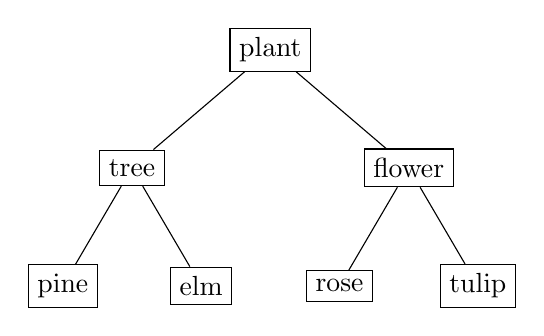
\begin{tikzpicture}[
  every node/.style = {shape=rectangle, draw, align=center},
   level 1/.style={sibling distance=10em},
   level 2/.style={sibling distance=5em}
    ]
  \node {plant}
    child { node {tree}
      child { node {pine} }
      child { node {elm} } }
    child { node {flower}
      child { node {rose} }
      child { node {tulip} } };
\end{tikzpicture}
\end{center}
\caption{Example conceptual tree}
\end{figure}


\begin{figure}[hbt]
\begin{center}
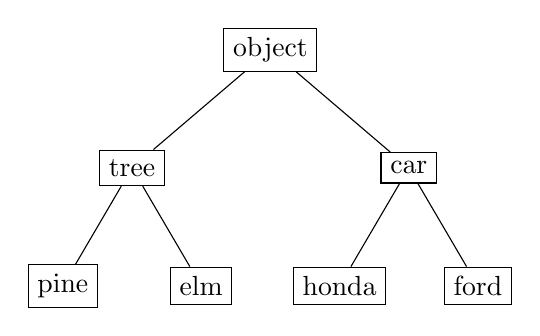
\begin{tikzpicture}[
  every node/.style = {shape=rectangle, draw, align=center},
   level 1/.style={sibling distance=10em},
   level 2/.style={sibling distance=5em}
    ]
  \node {object}
    child { node {tree}
      child { node {pine} }
      child { node {elm} } }
    child { node {car}
      child { node {honda} }
      child { node {ford} } };
\end{tikzpicture}
\end{center}
\caption{Alternative set of relationships}
\end{figure}

Rosch and others went on to show that culture and environment can effect what individuals come to understand as \say{prototypical}; in other words, how they come to distinguish experience.
For an individual raised in a forest, for example, the categories of \textit{pine} and \textit{elm} may in fact be prototypical categories.
For this individual, the differences between the two species are more salient than their similarities.
We can see this also in many professions: professionals communicate in jargon, making distinctions unfamiliar to those outside their field.

Rosch's work sheds a clarifying light on the relational nature of concepts.
What distinguishes \textit{tree} from \textit{elm} is not any particular property of \textit{elm}, but rather the presence of \textit{pine}.
If \textit{pine} did not exist, then \textit{elm} would add no information above and beyond that provided by \textit{tree}; \textit{elm} would not even exist.

American cognitive linguist George Lakoff develops Rosch's ideas in new directions, making central the idea of \textit{metaphor} in building understanding \cite{lakoff03}.
In Lakoff's view, complex ideas (distinctions) are understood by analogy from more basic ideas (distinctions).
A child, for instance, first comes to understand ideas of \textit{up} and \textit{down}, and \textit{warm} and \textit{cold}.
These first ideas are rooted in physical experience (the child has a body and experiences physical phenomena).
The child later comes to associate warmth with affection and cold with rejection (by observing the relationship between physical warmth and closeness to a parent, for example).

Once established, a child can come to understand more complex ideas by seeing them in terms of the more basic metaphors.
For example, imagine a child coming to understand a tumultuous friendship through the ideas of \say{hot} and \say{cold}.
For example, imagine a couple coming to understand their relationship as a journey they are on together.
The metaphoric nature of our understanding shapes politics, Lakoff argues: candidates shape messages and choose words with care in their attempt to create advantageous associations in the minds of the electorate \cite{lakoff14}.

With these examples, we wish to show that the principles of distinction and opposition developed with regards to the dialectic can be applied more generally to mundane and everyday concepts.

\subsubsection{A Thought Experiment}

As a thought experiment, let's imagine a new intelligent agent, such as a human infant, or some hypothetical AI, has just come into existence.
Having been instantiated without assumptions, this agent possesses just one single, unified concept, extending infinitely in all directions.

The agent begins to experience a constant stream of stimulus, and must somehow learn how to navigate and act in the environment. What might this agent do? What operations are possible?

If the agent's entire understanding consists of a single concept, then the first thing the agent might do it \textbf{separate} that concept into two concepts.
The separation might be along some \textbf{dimension}, such that the two resulting concepts exist in some relation to each other.
Having successfully performed the separate operation, the agent could separate the resulting concepts again and again, recursively ad infinitum, each time along some new dimension, achieving an arbitrarily refined conceptual structure.

In understanding the \textbf{separate} operation, we have the notion of dimension.
Recalling Lakoff's basic metaphor, an early separation could be between left and right, or up and down -- basic distinctions needed to navigate physical environments.
As each separation is performed in sequence, we can also imagine a \textit{hierarchy} of separations, with earlier separations representing more fundamental distinctions, with later separations representing more fine-grained distinctions (within the framework established by earlier separations).

As a brief digression, it is thought-provoking to imagine this process of recursive conceptual definition as a sort of inverse of a traditional Buddhist or Hindu meditation practice.
In a meditation practice, one attempts to cease making distinctions in their experience. Here, we intentionally develop a system of distinctions recursively out of undifferentiated experience.


\subsection{Ordering and Pairwise Preference}

If we exhibit prejudice towards numerical representation, what alternatives might there be? Any candidate representation should exhibit the following desiderata:

\begin{enumerate}
  \item The space between objects is left undefined.
\end{enumerate}

Fortunately, item \textit{ordering} makes no statement about the nature of the relationship between the items, apart from their relative relations to each other.

\bigskip

Nobel prize-winning economist Kenneth Arrow has done extensive work analyzing voting systems.
Throughout much of his career, he advocated for ordinal representation of preference \cite{bianchi}, pointing out that relative preference is all that is naturally observed:

\begin{center}
	\begin{quotation}
\textit{
	The only evidence of an individual's utility function is supplied by his observable behavior, specifically the choices he makes in the course of maximizing the function.
	But such choices are defined by the preference order and must therefore be the same for all utility functions compatible with that ordering.
	\textbf{Hence there is no quantitative meaning of utility for an individual.}
	}
\end{quotation}
- Kenneth Arrow 1973; p104, emphasis added
\end{center}

However, Arrow would also show the limits of such a representation.
In his \textit{impossibility theorem}, Arrow proved that no ranked-choice system could satisfy all of a set of voting system criteria \cite{arrow}.
In light of this, Arrow would later amend his views and come to tolerate cardinal representations of preference, which contemplate real-valued distance between items, on the grounds that such representations provide additional information \cite{hamlin}.
Indeed, certain limitations of ordinal preference representation (such as the possibility of intransitive preference) are absent given cardinal preference representation.
However, Arrow cautioned against such systems, observing that wide ranges made it more likely that voters would misrepresent their preferences \cite{hamlin}:  \say{The trouble with methods where you have three or four classes, I think if people vote sincerely they may well be very satisfactory. The problem is the incentive to misrepresent your vote may be high.}

Interpreting Arrow's comments through our framework of representation and measurement, it seems as though we can interpret cardinal preferences as capable of representing more information.
We can see this is the case, given that we can always convert cardinal preferences to ordinal, but not vice versa.

This would seem to be a challenge for this thesis, which has been prejudiced against numerical representation of subjectivity.
If the question was only general expressiveness of representation, then the challenge would be severe.
Arrow's comments on error, however, point to a deeper tension: measurement error is almost certain to be higher for cardinal representations.

Returning to our formalisms, if we denote ordinal measurements with $r_o$, cardinal measurements with $r_c$, and the reduction of cardinal measurements to ordinal with $g_{co}$, we see that:

\[
I(Y; r_c(Y)) \geq I(Y; g_{co}(r_c(Y)))
\]

but 

\[
I(Y; r_c(Y)) \stackrel{?}{=} I(Y; r_o(Y))
\]

The latter uncertainty is due to the unknown trade off between expressiveness and measurement error.

\bigskip

We argue that pairwise preference has the advantage of being able to \textit{directly represent} subjectivity: a preference (or distinction) between two concepts.
This property emerges from the structured and limited nature of the pairwise preference: two items, and a preference for one over the other.
This representation does not by itself contain a huge amount of information, but what information is contained is an accurate reflection of the aspect of the world being represented: subjective preference.
We argue that, due to this direct representation, pairwise preferences are robust against measurement error; using terminology developed earlier, we can think of a pairwise preference as having a proxy gap of near-zero.
Regarding potential intransitivity of preference, seen as a major weakness for ordinal preference representation, we contend that such intransitivity is a feature of subjective experience, and we and seek to develop methods for recognizing and responding to intransitivity.
In the parlance of software engineering, \say{it's not a bug, its a feature}.

It is exactly for this ability of pairwise preference to directly represent subjectivity (and the contradictions that sometimes appear) that we choose to explore it.